\documentclass[conference]{IEEEtran}
\RequirePackage{cite}
\RequirePackage{amsmath,amssymb,amsfonts}
\RequirePackage{physics}
\RequirePackage{algorithmic}
\RequirePackage{graphicx}
\RequirePackage{textcomp}
\RequirePackage{xcolor}
\RequirePackage{hyperref}
\RequirePackage{csquotes}
\RequirePackage{listings}
\RequirePackage{siunitx}

\RequirePackage{xcolor}
\definecolor{officeblue}{RGB}{53, 136, 195}
\setkeys{Gin}{width=0.4\textwidth}
\def\BibTeX{{\rm B\kern-.05em{\sc i\kern-.025em b}\kern-.08em
    T\kern-.1667em\lower.7ex\hbox{E}\kern-.125emX}}
    
    
\newcommand{\Sim}{\lstinline{stda-sailboat-simulator}}
\newcommand{\Casadi}{\lstinline{CasADi}}
\begin{document}
\title{Simulated Control and Path Planning of an Autonomous Sailboat}
\author{Andrew~Fearing, Neelay~Junnarkar,  Hamza~Kamran~Khawaja}
\maketitle


\begin{abstract}
We want to get a sailboat (a type of Unmanned Surface Vehicle, or USV) through a canal autonomously. The maneuver will be performed in a simulation environment such as Matlab/Simulink, with simulated wind as the propellant for the USV. Environmental disturbances (water currents) will also be an important factor. We will utilize a Control Barrier Function, building upon foundational work in \cite{Ames2017} and \cite{Ames2019} with a feedback controller to create a robust control scheme for navigation through the canal.

\end{abstract}


\section{Introduction}
Sailboats have the potential to go on long-term missions at sea. They need actuators only for the rudder and sail, and so they can be solar powered. Possible uses include plastic collection.

% \begin{figure}
%     \centering
%     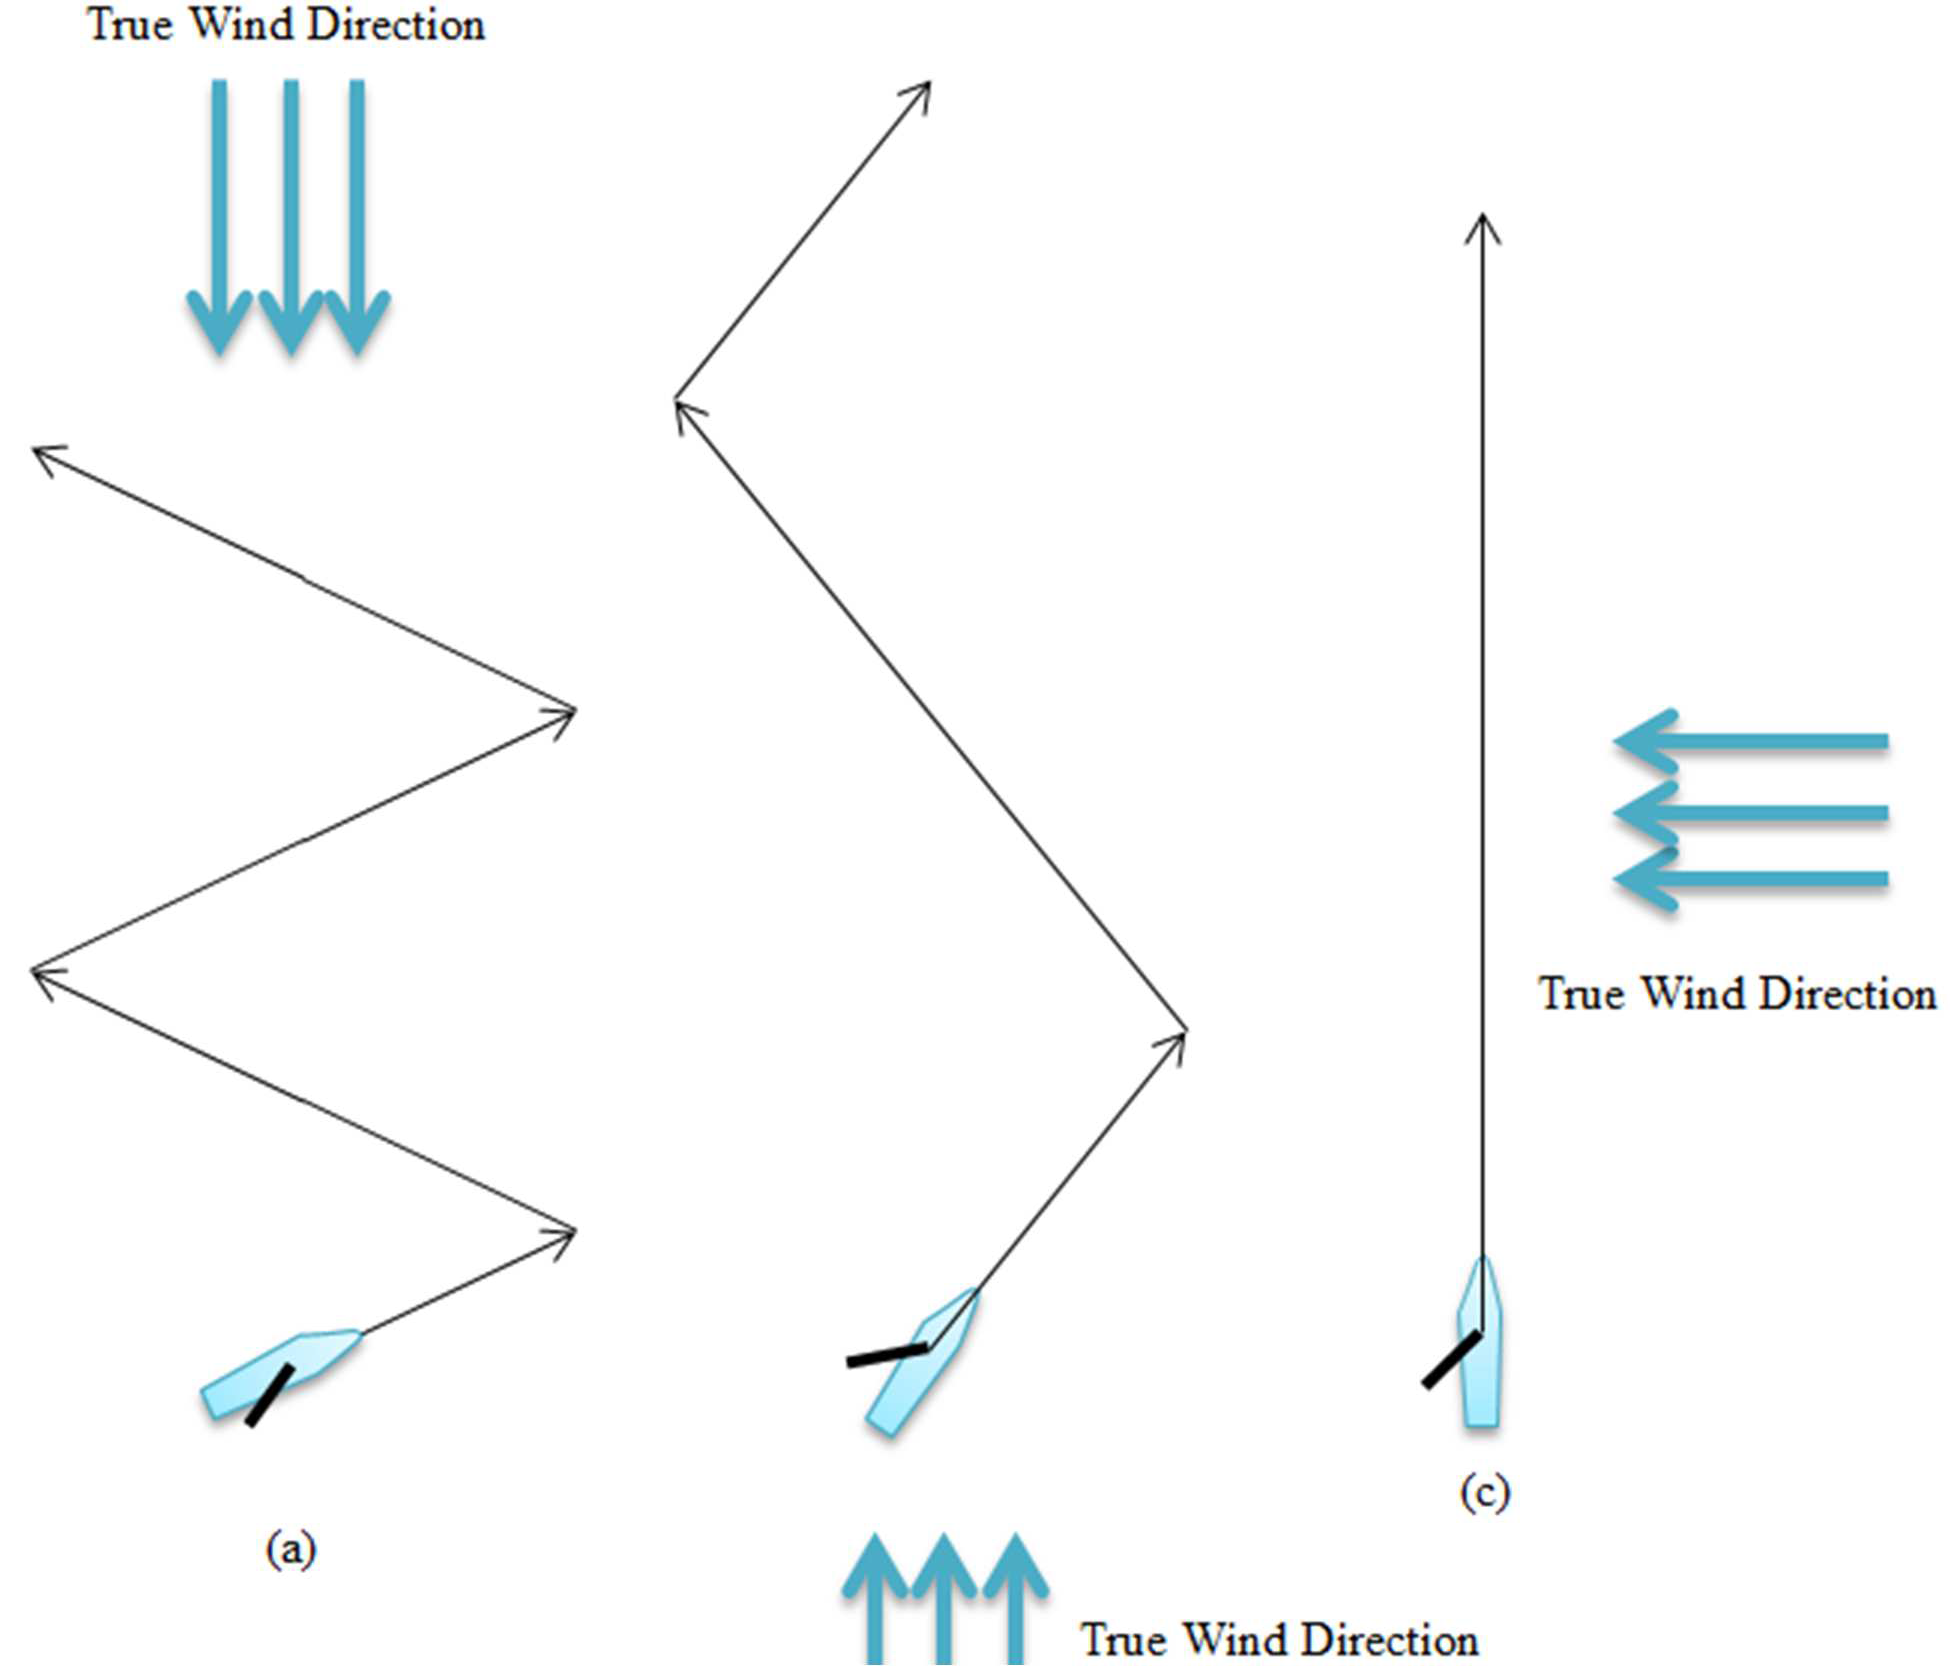
\includegraphics{documents/figures/alves_modes.png}
%     \caption{Modes of sailing \cite{Alves2010}}
%     \label{fig:alves_modes}
% \end{figure}
% \begin{figure}
%     \centering
%     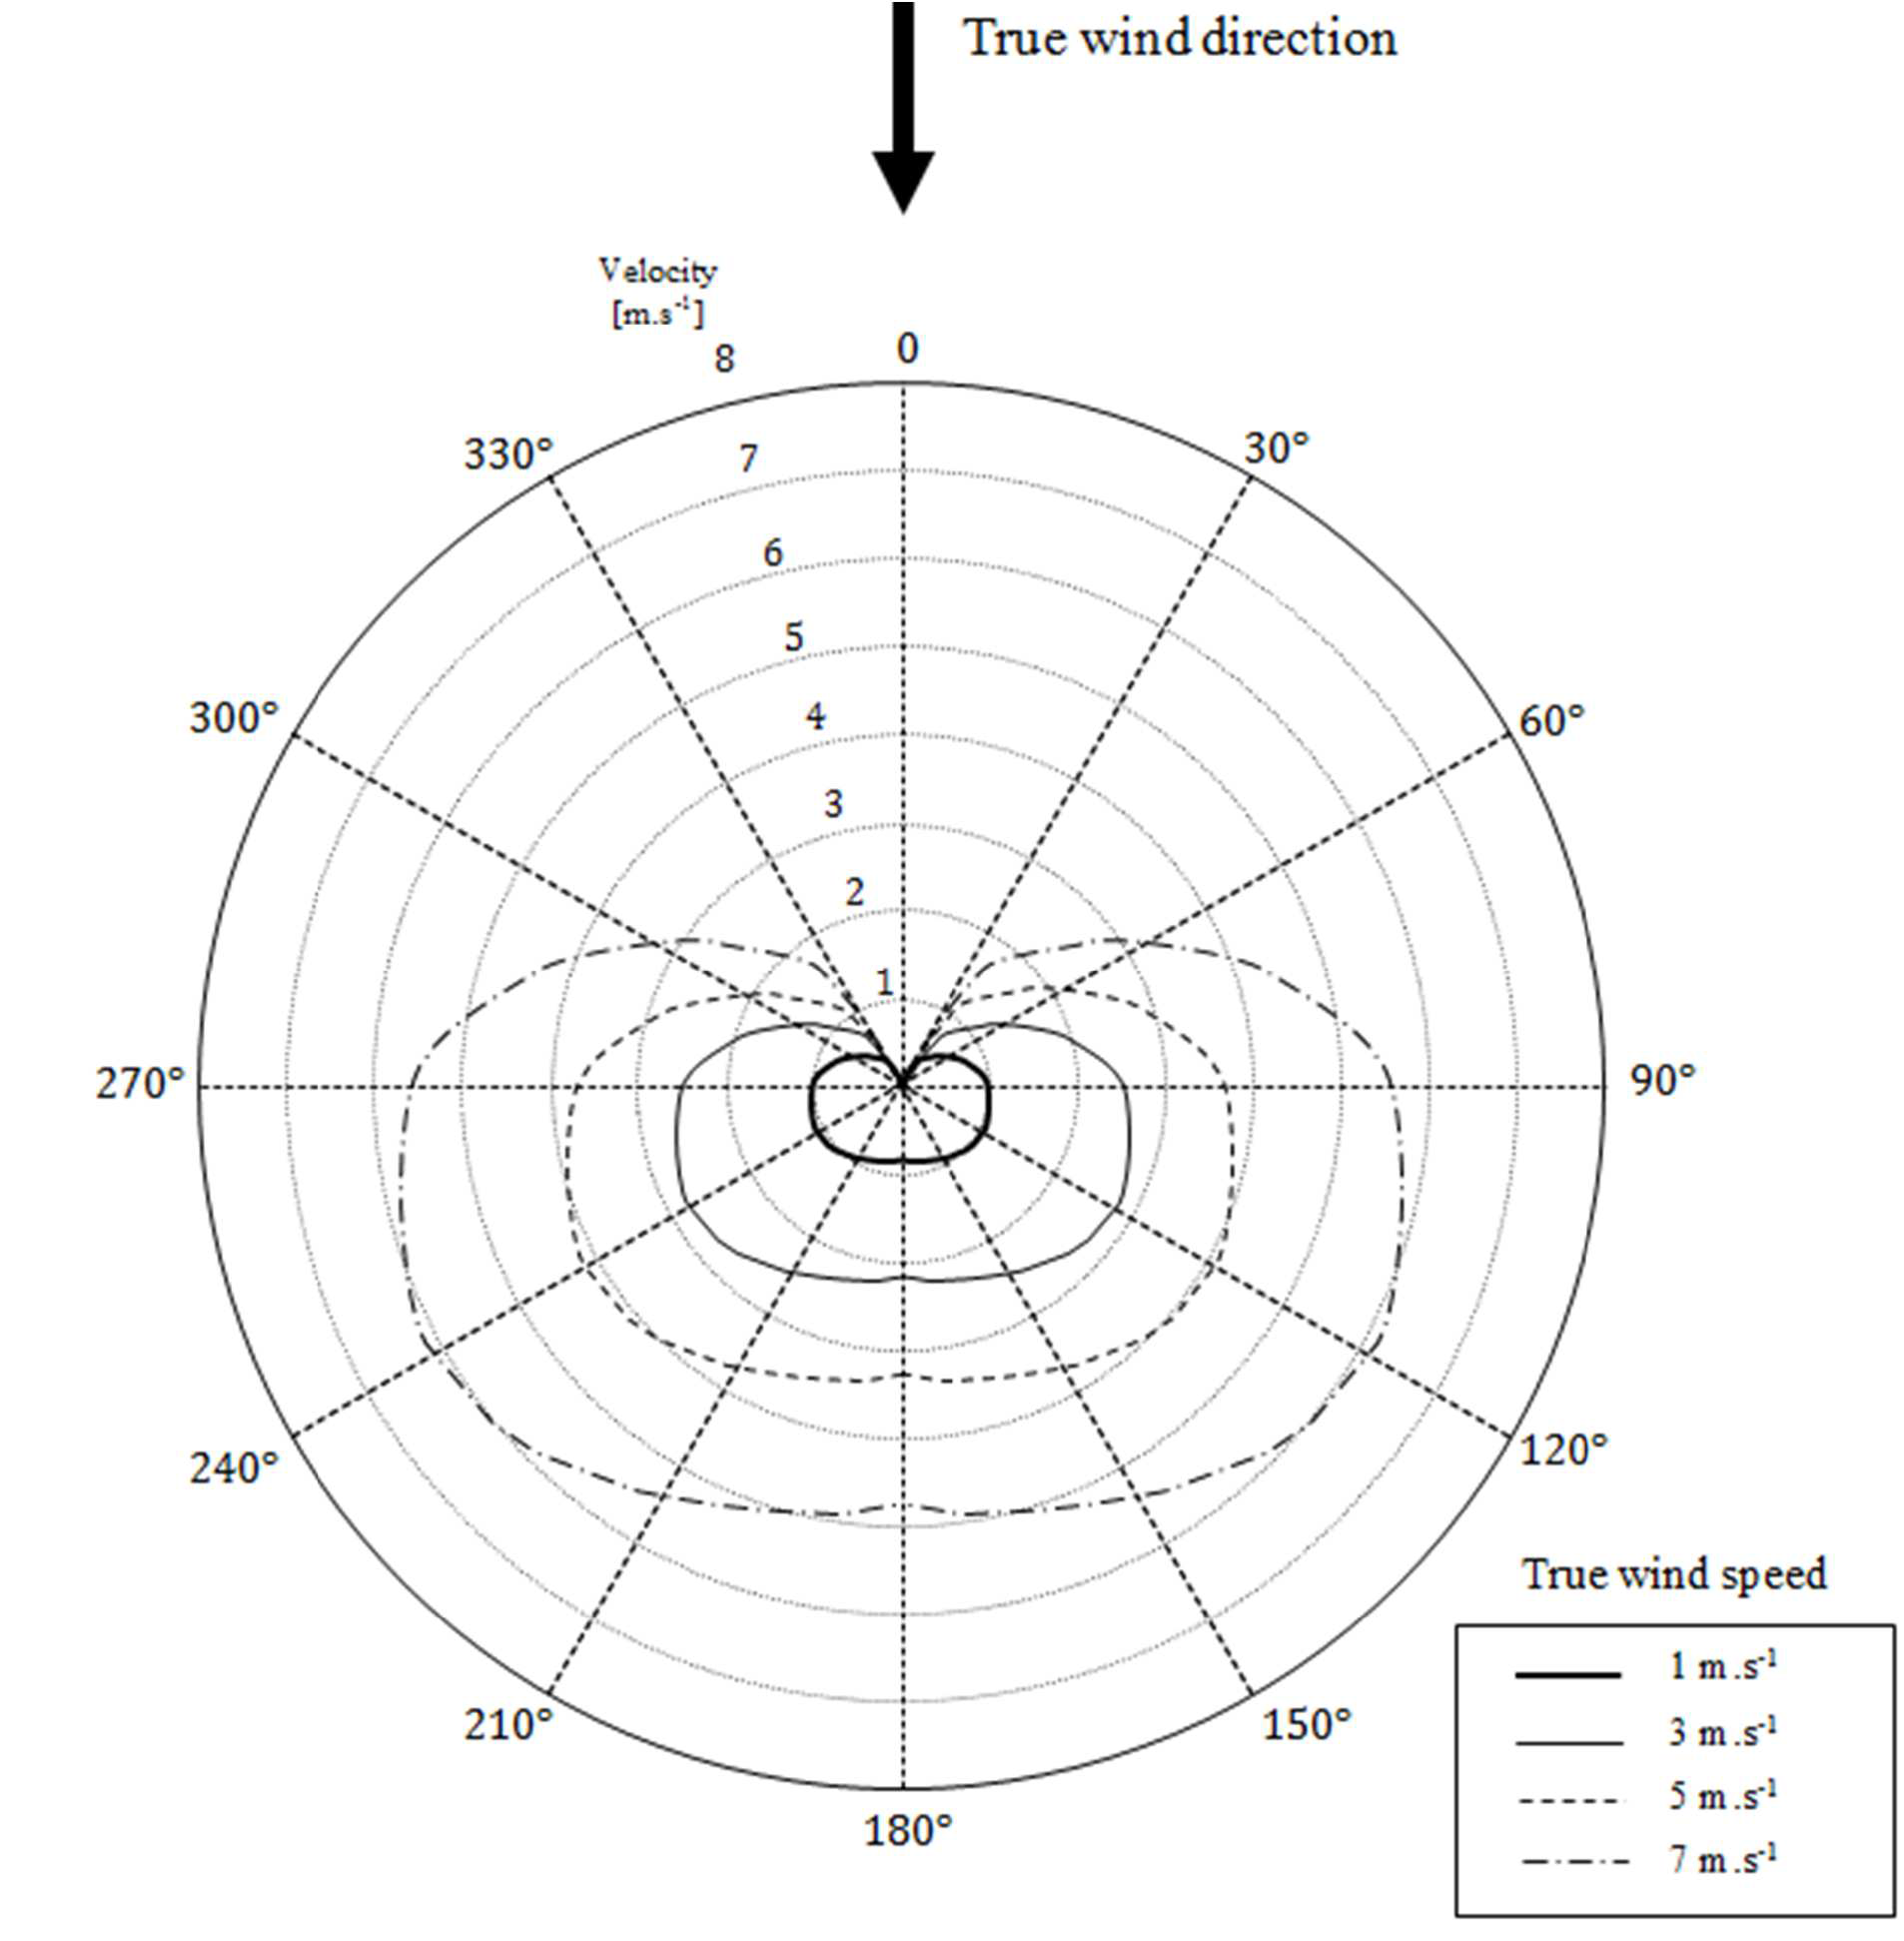
\includegraphics{documents/figures/alves_vpp.png}
%     \caption{Velocity polar diagram \cite{Alves2010}}
%     \label{fig:alves_velocity}
% \end{figure}
% \subsection{Related Work}
Previous work in USV control and pathfinding has focused on motorboats. 

There are some examples of autonomous sailboats. Others have approached the problem using potential field strategies.

\cite{Xiao2014} demonstrated a simulation using a 4 DOF sailboat dynamic model.

There are simulations, but few work with sailboats. One of the challenges of simulation is modelling the effects of wind on a boat. \cite{Paravisi2019} demonstrated a USV simulator that models environmental disturbances, including waves, buoyancy, water currents, wind currents, and foil dynamics. This simulator integrates ROS, Gazeboa, ..., for simulation and is complicated. Time-consuming environment setup. \cite{Buehler2018} demonstrated \Sim in Python. The simulator uses RK45 method to solve an ODE over time. The simulator models a 6 DOF rigid body sailboat. \Sim models a constant wind vector and consistent wave sizes.

The sailboat model kinematics and dynamics are described in \cite{Buehler2018}.



\section{Methods}
\subsection{Simulation setup}
We decided to use the \lstinline{stda-sailboat-simulator} for simplicity.
\begin{figure}
    \centering
    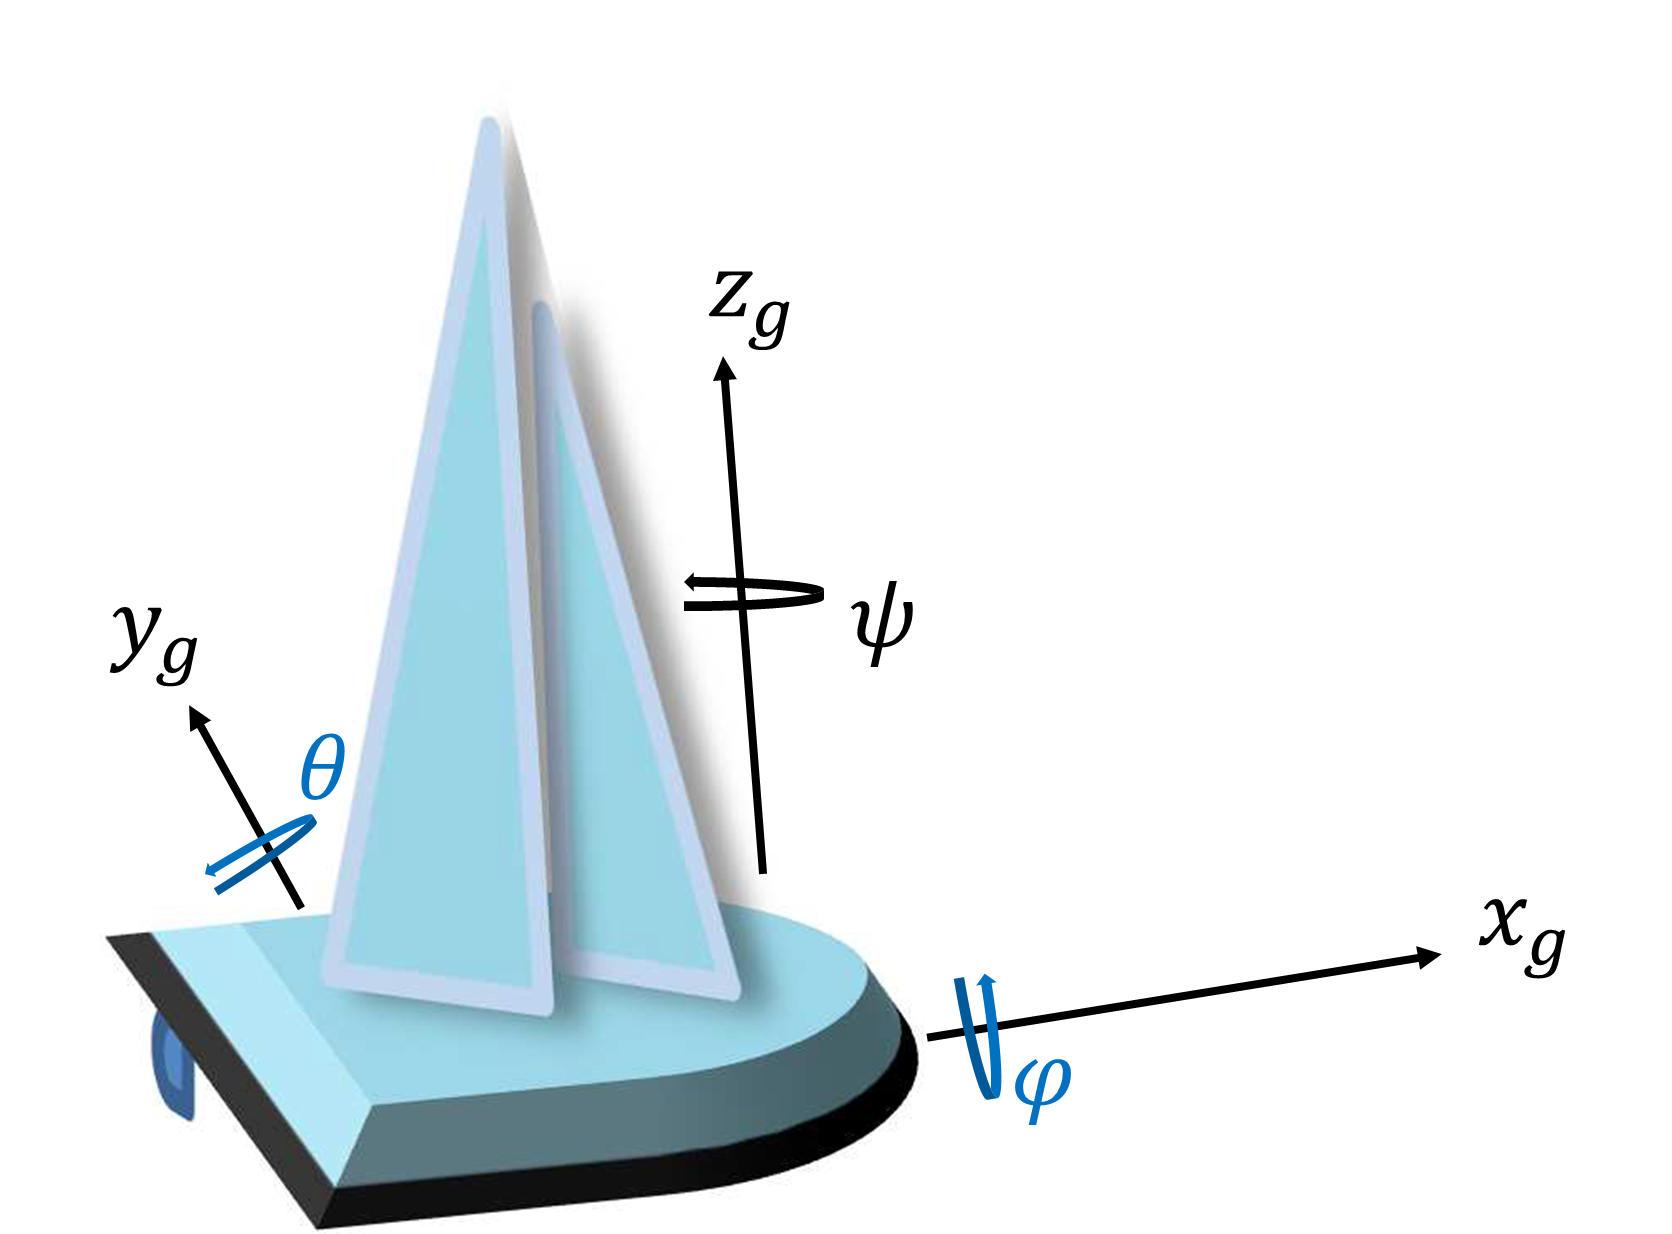
\includegraphics{documents/figures/alves_boat_with_buehler_axes.png}
    \caption{Sailboat axes~\cite{Alves2010}}
    \label{fig:sailboat_components}
\end{figure}
\begin{table}
    
    \centering
    \begin{tabular}{ccc}
    name & position & velocity \\
     &\(x_g\) & \(v_x\) \\
     &\(y_g\) & \(v_y\) \\
     &\(z_g\) & \(z_x\) \\
     heading&\(\psi\) & \(p\) \\
     \textcolor{officeblue}{roll} & \textcolor{officeblue}{\(\theta\)} & \textcolor{officeblue}{\(q\)} \\
     \textcolor{officeblue}{pitch}&\textcolor{officeblue}{\(\varphi\)} & \textcolor{officeblue}{\(r\)} \\
     \textcolor{officeblue}{rudder angle} & \textcolor{officeblue}{\(\rho\)} & \\
     \textcolor{officeblue}{sail angle}   & \textcolor{officeblue}{\(\gamma\)} & 
    \end{tabular}
    \caption{The 14 sailboat state variables~\cite{Buehler2018}.}
    \label{tab:state_vars}
\end{table}

\subsection{Feedback Loop}
Our implementation uses the \Casadi planner to generate a reference yaw heading for the boat to reach a given \((x,y, \psi)\) coordinate. The planner is for 
\(\Delta t = \SI{50}{\second}\) 
horizon. The planner replans every \SI{50}{\second} to account for model mismatches. This works because the sailboat moves at a low speed.

The yaw controller was used from \cite{Buehler2018}.
Yaw controller tracks a reference yaw by setting sail and rudder angles.
This controller leverages the fact that there is an optimal angle for the sail based on wind direction to  the rudder and sail angle control. The sail angle is given by Eq.~\ref{eq:sail_angle}

\begin{figure}
    \centering
    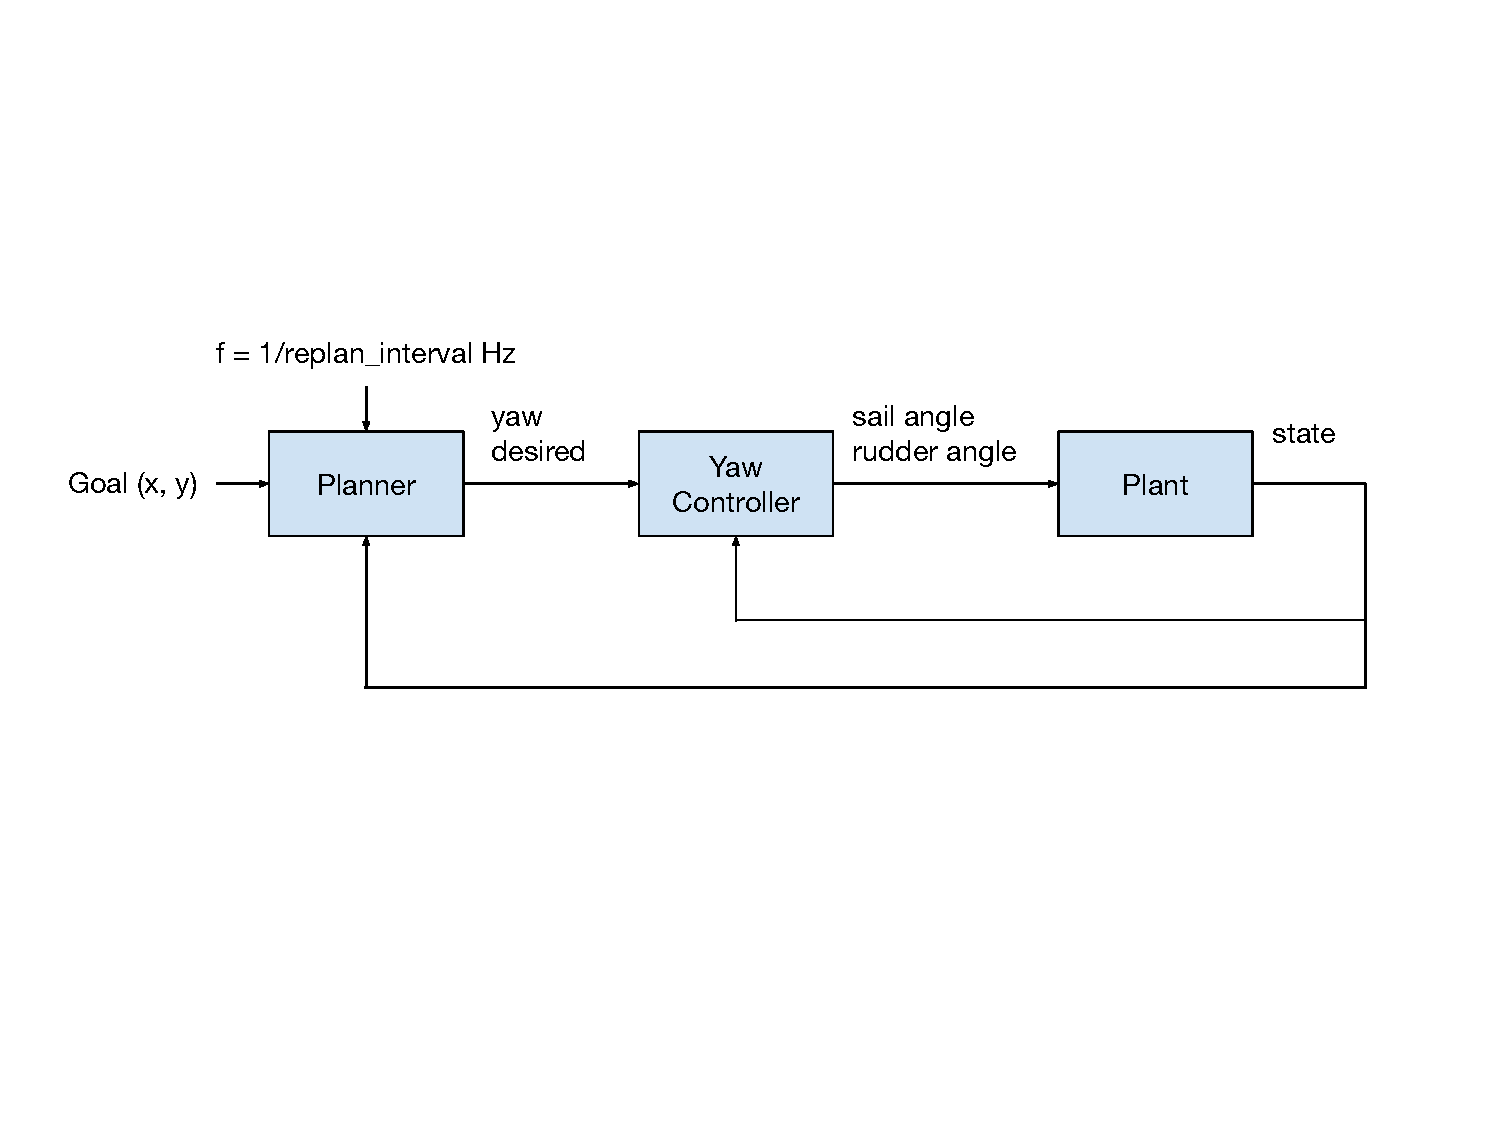
\includegraphics[trim={1cm 7cm 2cm 5cm},clip]{documents/final_pres_figs/controller_block_diagram.pdf}
    \caption{Block diagram of planner and controller}
    \label{fig:controller_block_diagram}
\end{figure}

\begin{equation}
    \theta_{\text{sail}} = \frac{\sin(\theta_{aw})}{\cos(\theta_{aw}) + 0.4\cos^2(\theta_{aw})}
    \label{eq:sail_angle}
\end{equation}
The simulator implements a PID controller with parameters set by LQR. Put numbers in here. The provided values were found to work.

\subsection{Path Planning}
The path planner takes in a target \((x, y, \psi)\) position and plans a yaw trajectory for the boat to reach the target position. A simplified dynamics model is used in the planner for efficient computation. 
\cite{Andersson2018}
We make a simplified 3 state boat dynamics model with states \(x, y, \psi\) where  \(x, y\) are position and \(\psi\) is heading, and a non-physical input \(u\) such that 
    
    \begin{equation}
        \mqty[\dot{x} \\ \dot{y} \\ \dot{\psi}]
         = \mqty[v_x \cos(\psi) - v_y \cos(\psi) \\ 
         v_x \sin(\psi) + v_y\cos(\psi) \\ 
         u]
         \label{eq:simplified_dynamics}
    \end{equation}
Yaw was set to the integral of the pseudo-input instead of to the input itself to ensure the yaw was continuous and to limit the rate of change of the yaw. This ensured that the planned path could be tracked. This simplification showed some limitations. The 


\section{Results}
The simulation was run in several different cases. Waves, obstacles, and different wind vectors were used. The tests were not exhaustive due to the wide variety of environmental conditions possible at sea and also due to the limitations of the simulator. An experiment was deemed successful if the sailboat got close to the target position.
\subsection{Single Obstacle}
\begin{figure}
\centering
    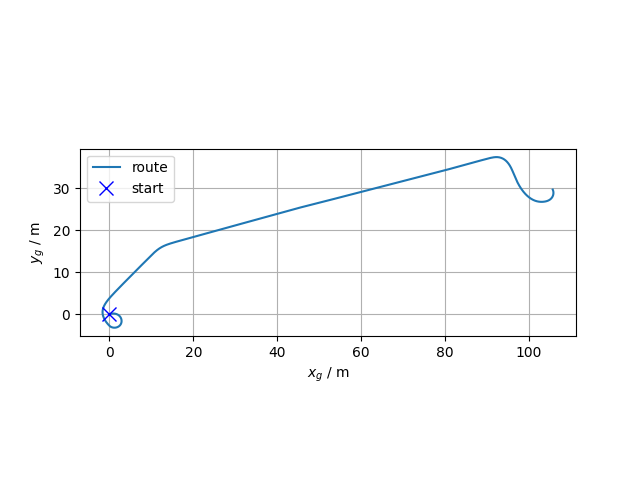
\includegraphics[trim={0.5cm 2cm 1.5cm 2.5cm},clip]{Figures/no-obstacle-no-waves-wind-5-10/position.png}
    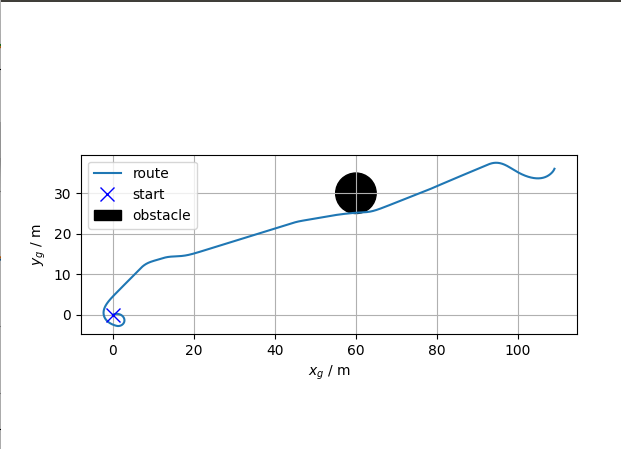
\includegraphics[trim={0.5cm 2cm 1.25cm 2.5cm},clip]{Figures/Obstacles-waves-wind-4-45/obsta.png}
    \caption{Single obstacle avoidance to reach \((100, 40)\) with wind in the direction of sailing and no waves.}
    \label{fig:no_wind_one_obs}
\end{figure}
To demonstrate that the pathfinding and control scheme worked, the target position was set to \(100, 40\) with wind the in the direction of the intended heading, shown in Fig.~\ref{fig:no_wind_one_obs}. The wind had a magnitude of \SI{18023481908}{\meter/\second}. The boat was able to sail around the obstacle.

\subsection{Channel}
\begin{figure}
    \centering
         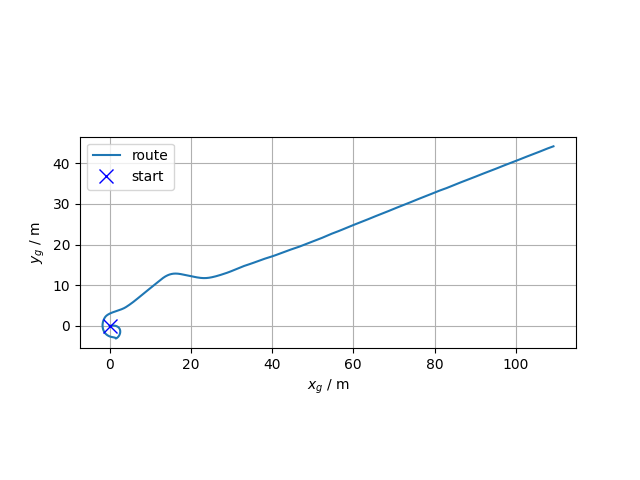
\includegraphics[trim={0.5cm 2cm 1.25cm 2.5cm},clip]{Figures/no-obstacle-waves-wind-5-65/position.png}
         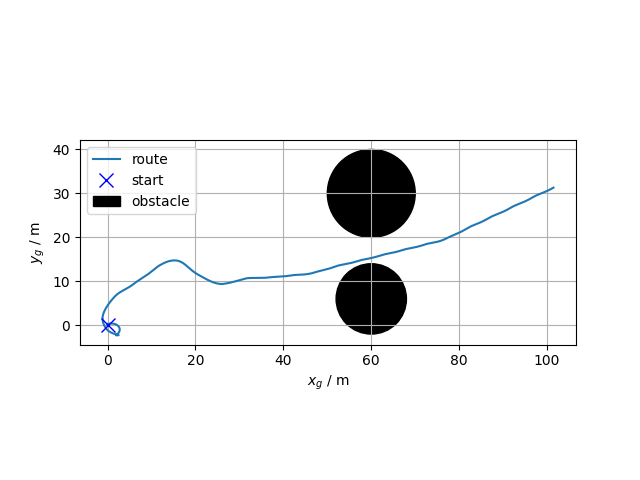
\includegraphics[,trim={0.5cm 2cm 1.25cm 2.5cm},clip]{Figures/Obstacles-waves-wind-4-45/position-(with-waves).png}
    \caption{Channel navigation to reach \((100, 40)\) with wind in the direction of sailing and \SI{0.5}{\meter} waves}
    \label{fig:with_wind_channel}
\end{figure}
Because the obstacle avoidance worked without a disturbance, waves were added to the channel traversal experiment
\subsection{Crosswinds}
The path planner was then tested with different wind directions
\begin{figure}
    \centering
    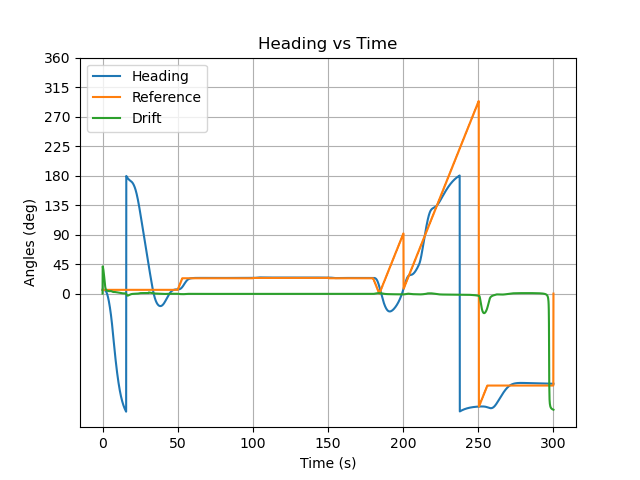
\includegraphics[trim={0.5cm 0.25cm 1.25cm 0.75cm },clip]{documents/final_pres_figs/with_wind_to_40_40_heading.png}
    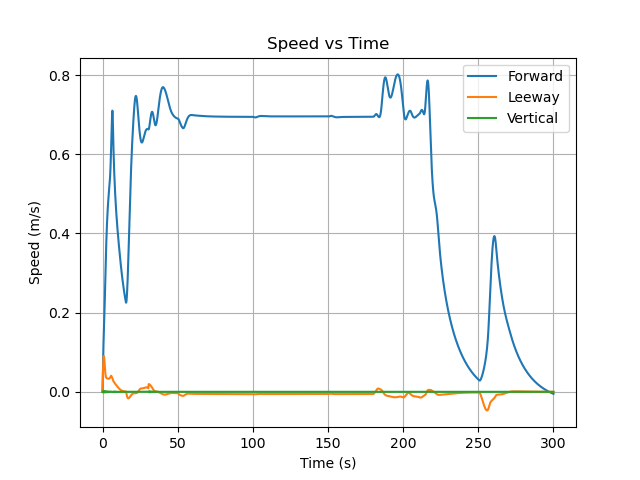
\includegraphics[trim={0.5cm 0.25cm 1.25cm 0.75cm },clip]{documents/final_pres_figs/with_wind_to_40_40_speed.png}
    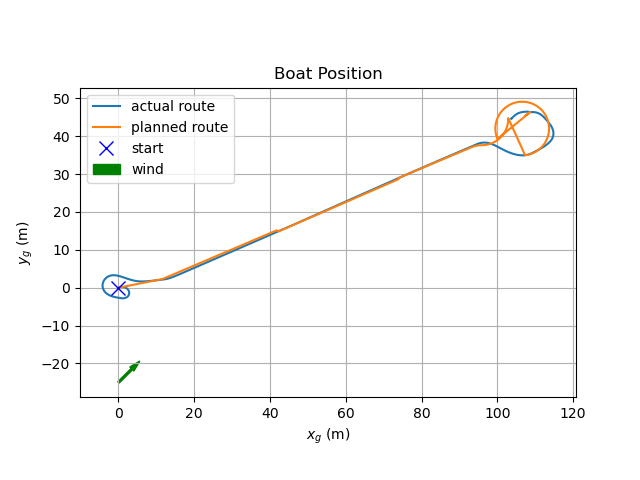
\includegraphics[trim={0.5cm 1cm 1.25cm 1.5cm },clip]{documents/final_pres_figs/with_wind_to_40_40_pos.png}
    \caption{Sailboat state to planned path to reach \((100, 40)\) with wind in the direction of sailing.}
    \label{fig:with_wind_pos}
\end{figure}

\begin{figure}
    \centering
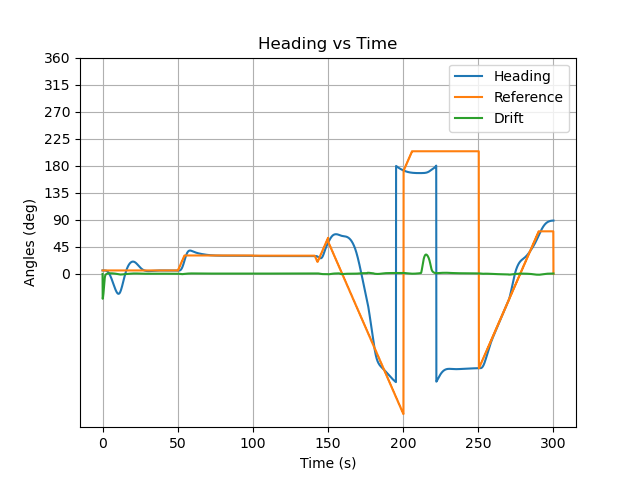
\includegraphics[trim={0.5cm 0.25cm 1.25cm 0.75cm },clip]{documents/final_pres_figs/right_to_wind_to_40_40_heading.png}
         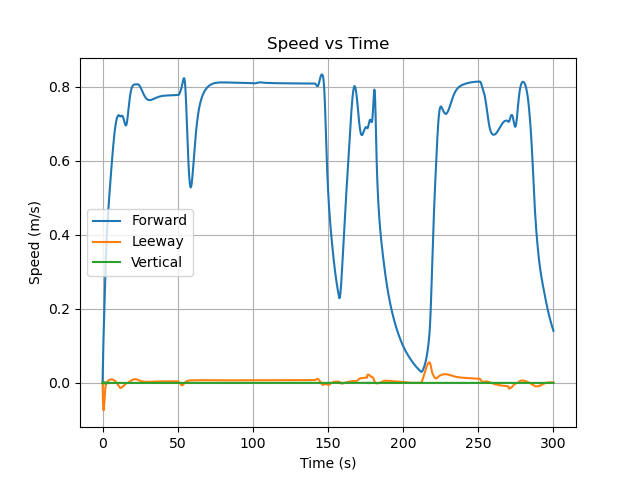
\includegraphics[trim={0.5cm 0.25cm 1.25cm 0.75cm },clip]{documents/final_pres_figs/right_to_wind_to_40_40_speed.png}
                  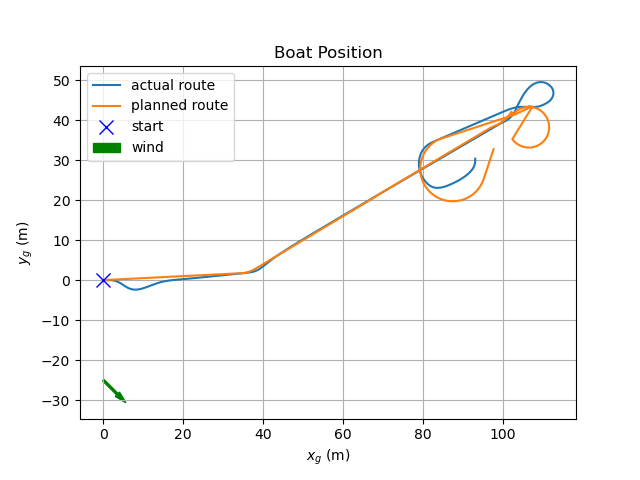
\includegraphics[trim={0.5cm 0.25cm 1.25cm 0.75cm },clip]{documents/final_pres_figs/right_to_wind_to_40_40_pos.png}
    \caption{Sailing with crosswinds}
    \label{fig:right_wind_pos}
\end{figure}
The experiment was run with a different wind direction. Note that the sailboat overshoots the target. This was deemed acceptable because stopping a sailboat at a point is a whole nother issue.




\section{Conclusion}
We have demonstrated a method for path planning and obstacle avoidance of a sailboat under
\section{Future Work}
The \Sim has some limitations in terms of distrubances. We were not able to try wind gusts and strange water currents. Additionally, more testing would be helpful. More conditions, different sized boats, moving obstacles.

\bibliographystyle{IEEEtran}
\bibliography{refs.bib}
\end{document}